% Generated type C_3 word-level weave Delta Delta -> Delta.
% Exact shortest trace: 32 local moves.
% Vertex counts: 9 contractions, 7 six-valent vertices,
% 6 eight-valent vertices; the 10 commutations are unmarked
% intersections of straight strands.
\begingroup
\colorlet{cThreeTeal}{teal!70!black}
\colorlet{cThreeOrange}{orange!82!black}
\colorlet{cThreeBlue}{blue!68!black}

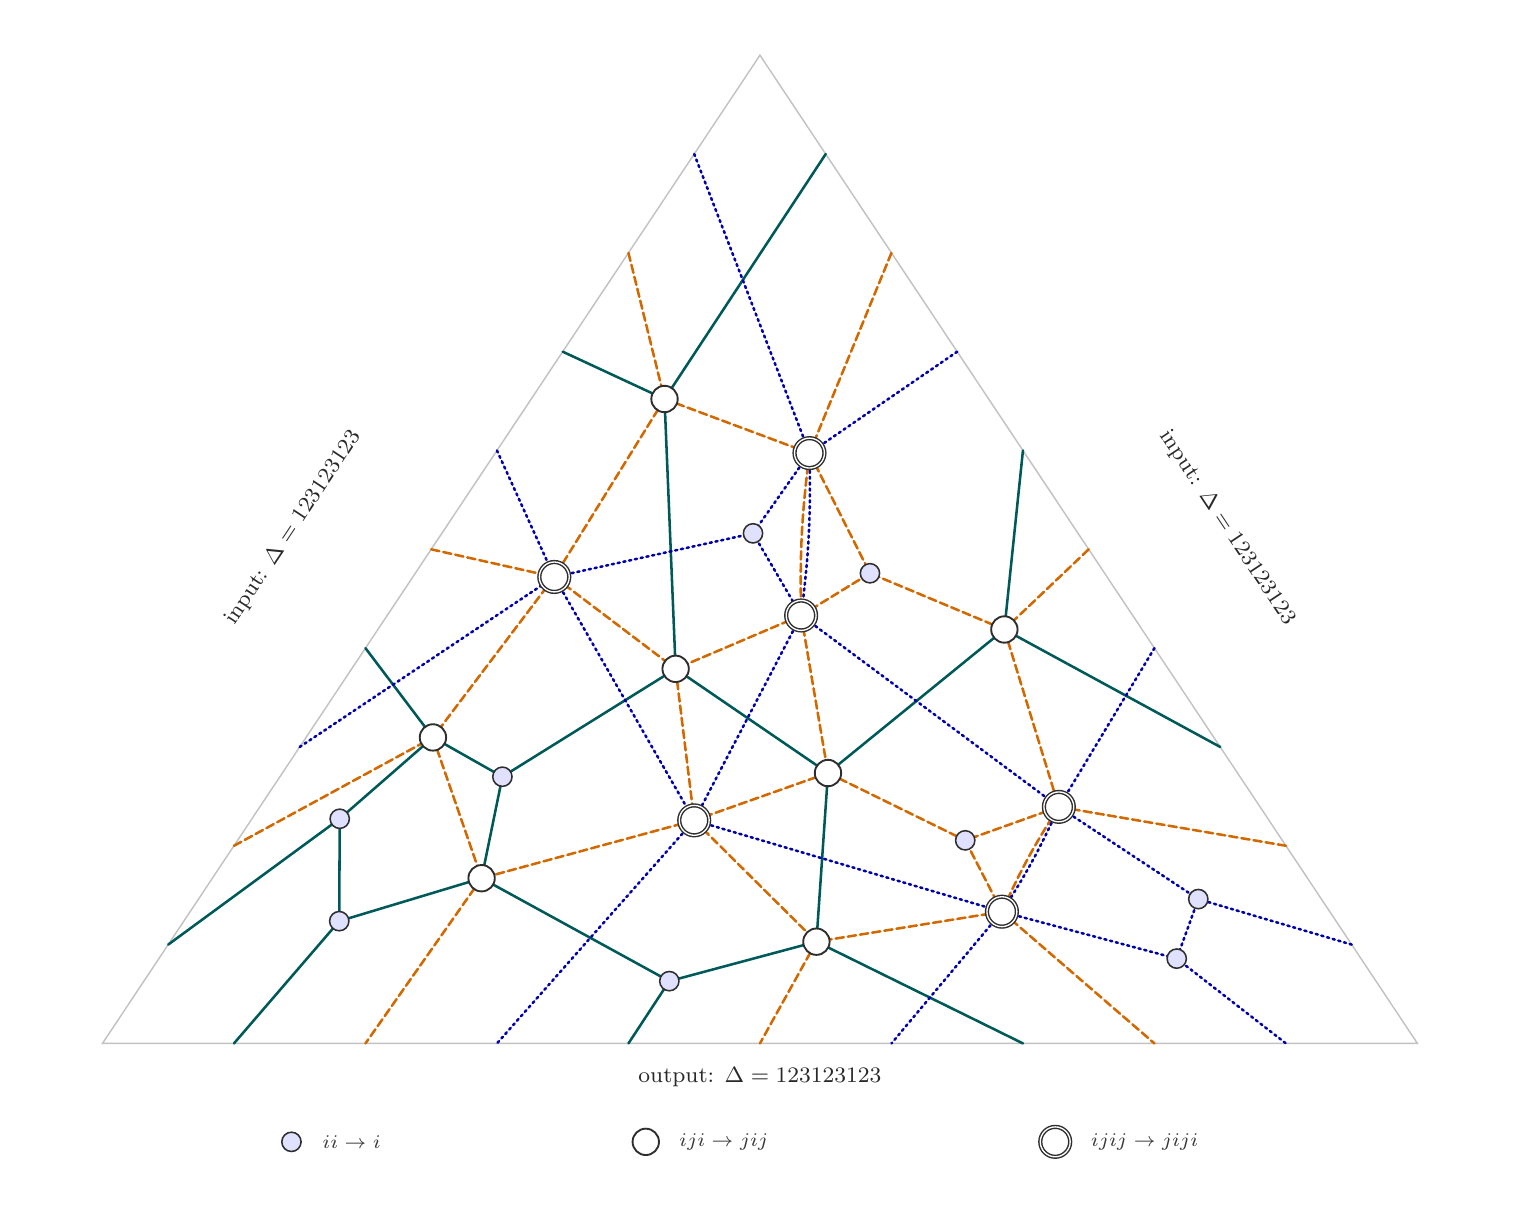
\begin{tikzpicture}[
  x=1cm,y=1cm,
  cThreeStrand/.style={line width=0.92pt,line cap=round,line join=round},
  cThreeOne/.style={cThreeStrand,draw=cThreeTeal},
  cThreeTwo/.style={cThreeStrand,draw=cThreeOrange,
    dash pattern=on 3.0pt off 1.45pt},
  cThreeThree/.style={cThreeStrand,draw=cThreeBlue,
    dash pattern=on 0.78pt off 1.35pt},
  cThreeFrame/.style={draw=black!24,line width=0.52pt},
  cThreeContraction/.style={circle,draw=black!82,fill=blue!12,
    minimum size=2.45mm,inner sep=0pt,line width=0.56pt},
  cThreeBraidThree/.style={circle,draw=black!82,fill=white,
    minimum size=3.35mm,inner sep=0pt,line width=0.68pt},
  cThreeBraidFour/.style={circle,draw=black!82,fill=white,double,
    double distance=0.48pt,minimum size=3.80mm,inner sep=0pt,
    line width=0.52pt},
  cThreeBoundary/.style={font=\footnotesize,fill=white,
    inner xsep=1.2pt,inner ysep=0.7pt,text=black!84},
  cThreeLegend/.style={font=\scriptsize,text=black!78}
]
\path[use as bounding box] (-9.30,-1.82) rectangle (9.30,12.90);
\coordinate (leftCorner) at (-8.350,0);
\coordinate (topCorner) at (0,12.550);
\coordinate (rightCorner) at (8.350,0);
\draw[cThreeFrame] (leftCorner)--(topCorner)--(rightCorner)--cycle;

% Strands are grouped by color.  A transverse crossing without a
% marker is a commutation of colors 1 and 3.
% Color 1 strands.
\draw[cThreeOne] (-5.010,5.020) -- (-4.153,3.886);
\draw[cThreeOne] (0.835,11.295) -- (-1.212,8.184);
\draw[cThreeOne] (-2.505,8.785) -- (-1.212,8.184);
\draw[cThreeOne] (-7.515,1.255) -- (-5.337,2.853);
\draw[cThreeOne] (-4.153,3.886) -- (-5.337,2.853);
\draw[cThreeOne] (-1.212,8.184) -- (-1.071,4.757);
\draw[cThreeOne] (5.845,3.765) -- (3.104,5.257);
\draw[cThreeOne] (3.340,7.530) -- (3.104,5.257);
\draw[cThreeOne] (-1.071,4.757) -- (-3.271,3.387);
\draw[cThreeOne] (-4.153,3.886) -- (-3.271,3.387);
\draw[cThreeOne] (3.104,5.257) -- (0.864,3.434);
\draw[cThreeOne] (-1.071,4.757) -- (0.864,3.434);
\draw[cThreeOne] (-3.271,3.387) -- (-3.535,2.098);
\draw[cThreeOne] (-5.337,2.853) -- (-5.343,1.553);
\draw[cThreeOne] (-3.535,2.098) -- (-5.343,1.553);
\draw[cThreeOne] (0.864,3.434) -- (0.717,1.292);
\draw[cThreeOne] (-3.535,2.098) -- (-1.151,0.791);
\draw[cThreeOne] (0.717,1.292) -- (-1.151,0.791);
\draw[cThreeOne] (0.717,1.292) -- (3.340,0.000);
\draw[cThreeOne] (-5.343,1.553) -- (-6.680,0.000);
\draw[cThreeOne] (-1.151,0.791) -- (-1.670,0.000);

% Color 2 strands.
\draw[cThreeTwo] (-1.670,10.040) -- (-1.212,8.184);
\draw[cThreeTwo] (-4.175,6.275) -- (-2.612,5.924);
\draw[cThreeTwo] (-1.212,8.184) -- (-2.612,5.924);
\draw[cThreeTwo] (-6.680,2.510) -- (-4.153,3.886);
\draw[cThreeTwo] (-2.612,5.924) -- (-4.153,3.886);
\draw[cThreeTwo] (-1.212,8.184) -- (0.629,7.497);
\draw[cThreeTwo] (1.670,10.040) -- (0.629,7.497);
\draw[cThreeTwo] (4.175,6.275) -- (3.104,5.257);
\draw[cThreeTwo] (0.629,7.497) -- (1.397,5.971);
\draw[cThreeTwo] (3.104,5.257) -- (1.397,5.971);
\draw[cThreeTwo] (0.629,7.497) to[bend left=-4.20] (0.523,5.435);
\draw[cThreeTwo] (1.397,5.971) -- (0.523,5.435);
\draw[cThreeTwo] (-2.612,5.924) -- (-1.071,4.757);
\draw[cThreeTwo] (0.523,5.435) -- (-1.071,4.757);
\draw[cThreeTwo] (3.104,5.257) -- (3.796,3.004);
\draw[cThreeTwo] (6.680,2.510) -- (3.796,3.004);
\draw[cThreeTwo] (0.523,5.435) -- (0.864,3.434);
\draw[cThreeTwo] (0.864,3.434) -- (2.607,2.579);
\draw[cThreeTwo] (3.796,3.004) -- (2.607,2.579);
\draw[cThreeTwo] (-1.071,4.757) -- (-0.835,2.833);
\draw[cThreeTwo] (0.864,3.434) -- (-0.835,2.833);
\draw[cThreeTwo] (-4.153,3.886) -- (-3.535,2.098);
\draw[cThreeTwo] (-0.835,2.833) -- (-3.535,2.098);
\draw[cThreeTwo] (2.607,2.579) -- (3.073,1.673);
\draw[cThreeTwo] (3.796,3.004) to[bend left=-4.20] (3.073,1.673);
\draw[cThreeTwo] (-0.835,2.833) -- (0.717,1.292);
\draw[cThreeTwo] (3.073,1.673) -- (0.717,1.292);
\draw[cThreeTwo] (-3.535,2.098) -- (-5.010,0.000);
\draw[cThreeTwo] (0.717,1.292) -- (0.000,0.000);
\draw[cThreeTwo] (3.073,1.673) -- (5.010,0.000);

% Color 3 strands.
\draw[cThreeThree] (-5.845,3.765) -- (-2.612,5.924);
\draw[cThreeThree] (-0.835,11.295) -- (0.629,7.497);
\draw[cThreeThree] (-3.340,7.530) -- (-2.612,5.924);
\draw[cThreeThree] (-2.612,5.924) -- (-0.088,6.478);
\draw[cThreeThree] (2.505,8.785) -- (0.629,7.497);
\draw[cThreeThree] (0.629,7.497) -- (-0.088,6.478);
\draw[cThreeThree] (5.010,5.020) -- (3.796,3.004);
\draw[cThreeThree] (-0.088,6.478) -- (0.523,5.435);
\draw[cThreeThree] (0.629,7.497) to[bend left=4.20] (0.523,5.435);
\draw[cThreeThree] (-2.612,5.924) -- (-0.835,2.833);
\draw[cThreeThree] (0.523,5.435) -- (3.796,3.004);
\draw[cThreeThree] (3.796,3.004) -- (5.567,1.833);
\draw[cThreeThree] (7.515,1.255) -- (5.567,1.833);
\draw[cThreeThree] (0.523,5.435) -- (-0.835,2.833);
\draw[cThreeThree] (-0.835,2.833) -- (3.073,1.673);
\draw[cThreeThree] (3.796,3.004) to[bend left=4.20] (3.073,1.673);
\draw[cThreeThree] (3.073,1.673) -- (5.293,1.077);
\draw[cThreeThree] (5.567,1.833) -- (5.293,1.077);
\draw[cThreeThree] (-0.835,2.833) -- (-3.340,0.000);
\draw[cThreeThree] (3.073,1.673) -- (1.670,0.000);
\draw[cThreeThree] (5.293,1.077) -- (6.680,0.000);

% Mark the noncommuting weave vertices after drawing the strands.
\node[cThreeBraidThree] (v03) at (-1.212,8.184) {};
\node[cThreeBraidFour] (v04) at (-2.612,5.924) {};
\node[cThreeBraidThree] (v05) at (-4.153,3.886) {};
\node[cThreeContraction] (v06) at (-5.337,2.853) {};
\node[cThreeBraidFour] (v08) at (0.629,7.497) {};
\node[cThreeContraction] (v09) at (-0.088,6.478) {};
\node[cThreeBraidThree] (v11) at (3.104,5.257) {};
\node[cThreeContraction] (v12) at (1.397,5.971) {};
\node[cThreeBraidFour] (v13) at (0.523,5.435) {};
\node[cThreeBraidThree] (v14) at (-1.071,4.757) {};
\node[cThreeContraction] (v16) at (-3.271,3.387) {};
\node[cThreeBraidFour] (v18) at (3.796,3.004) {};
\node[cThreeContraction] (v19) at (5.567,1.833) {};
\node[cThreeBraidThree] (v21) at (0.864,3.434) {};
\node[cThreeContraction] (v22) at (2.607,2.579) {};
\node[cThreeBraidFour] (v23) at (-0.835,2.833) {};
\node[cThreeBraidThree] (v24) at (-3.535,2.098) {};
\node[cThreeContraction] (v25) at (-5.343,1.553) {};
\node[cThreeBraidFour] (v27) at (3.073,1.673) {};
\node[cThreeContraction] (v28) at (5.293,1.077) {};
\node[cThreeBraidThree] (v30) at (0.717,1.292) {};
\node[cThreeContraction] (v31) at (-1.151,0.791) {};

% Boundary words are read counterclockwise: up the left side,
% down the right side, and from left to right along the bottom.
\node[cThreeBoundary,rotate=56.4] at (-5.93,6.55) {input: $\boldsymbol\Delta=123123123$};
\node[cThreeBoundary,rotate=-56.4] at (5.93,6.55) {input: $\boldsymbol\Delta=123123123$};
\node[cThreeBoundary] at (0,-0.43) {output: $\boldsymbol\Delta=123123123$};

% Legend for the three marked local moves.
\node[cThreeContraction] at (-5.95,-1.25) {};
\node[cThreeLegend,anchor=west] at (-5.68,-1.25) {$ii\to i$};
\node[cThreeBraidThree] at (-1.45,-1.25) {};
\node[cThreeLegend,anchor=west] at (-1.15,-1.25) {$iji\to jij$};
\node[cThreeBraidFour] at (3.75,-1.25) {};
\node[cThreeLegend,anchor=west] at (4.08,-1.25) {$ijij\to jiji$};
\end{tikzpicture}
\endgroup
